\documentclass[aspectratio=169]{beamer}
\usepackage[utf8]{inputenc}
\usepackage{graphicx}
\usepackage{amsmath}
\usepackage{booktabs}

% --- Theme and Layout Settings ---
\usetheme{Madrid}
\usecolortheme{default}

% REMOVE the footline and navigation symbols completely as requested
\setbeamertemplate{footline}{}
\setbeamertemplate{navigation symbols}{}

% --- Title Page Information ---
\title[FOC of 3-Phase IM]{Field Oriented Control (FOC) \\ for a 3-Phase Induction Motor}
\author{
    Surja Mondal (Roll No. 34901622011) \\
    Joydip Karmakar (Roll No. 34901622014) \\
    Angsu Priya Roy (Roll No. 34901622020) \\
    Hirak Sinha (Roll No. 34901622042) \\
    Keshab Sarkar (Roll No. 34901622044)
}
\institute{
    \textbf{Project Guide:} Prof. Deepjyoti Santra \quad \textbf{HOD:} Prof. Atanu Maji \\
    \vspace{0.3cm}
    Department of Electrical Engineering \\
    Cooch Behar Government Engineering College
}
\date{2026}

\begin{document}

% --- Slide 1: Title Page ---
\begin{frame}
    \titlepage
\end{frame}

% --- Slide 2: Introduction & Motivation ---
\begin{frame}{Introduction \& Motivation}
    \textbf{The Evolution of AC Motor Drives}
    \begin{itemize}
        \item \textbf{The Legacy of Scalar Control:} Traditional Constant Volts-per-Hertz ($V/f$) control governs only magnitude and frequency. It ignores spatial magnetic orientation, leading to sluggish transient responses and coupled torque/flux dynamics.
        \item \textbf{The FOC Paradigm Shift:} FOC (Vector Control) emulates the highly desirable, decoupled control dynamics of a separately excited DC motor within an AC machine.
        \item \textbf{Project Objective:} To systematically deconstruct and simulate an Indirect Field Oriented Control (IFOC) architecture for a 50 HP Squirrel-Cage Induction Motor using MATLAB/Simulink.
    \end{itemize}
\end{frame}

% --- Slide 3: System Architecture Overview ---
\begin{frame}{System Architecture Overview}
    \textbf{Top-Level IFOC Block Diagram}
    \begin{figure}
        \centering
        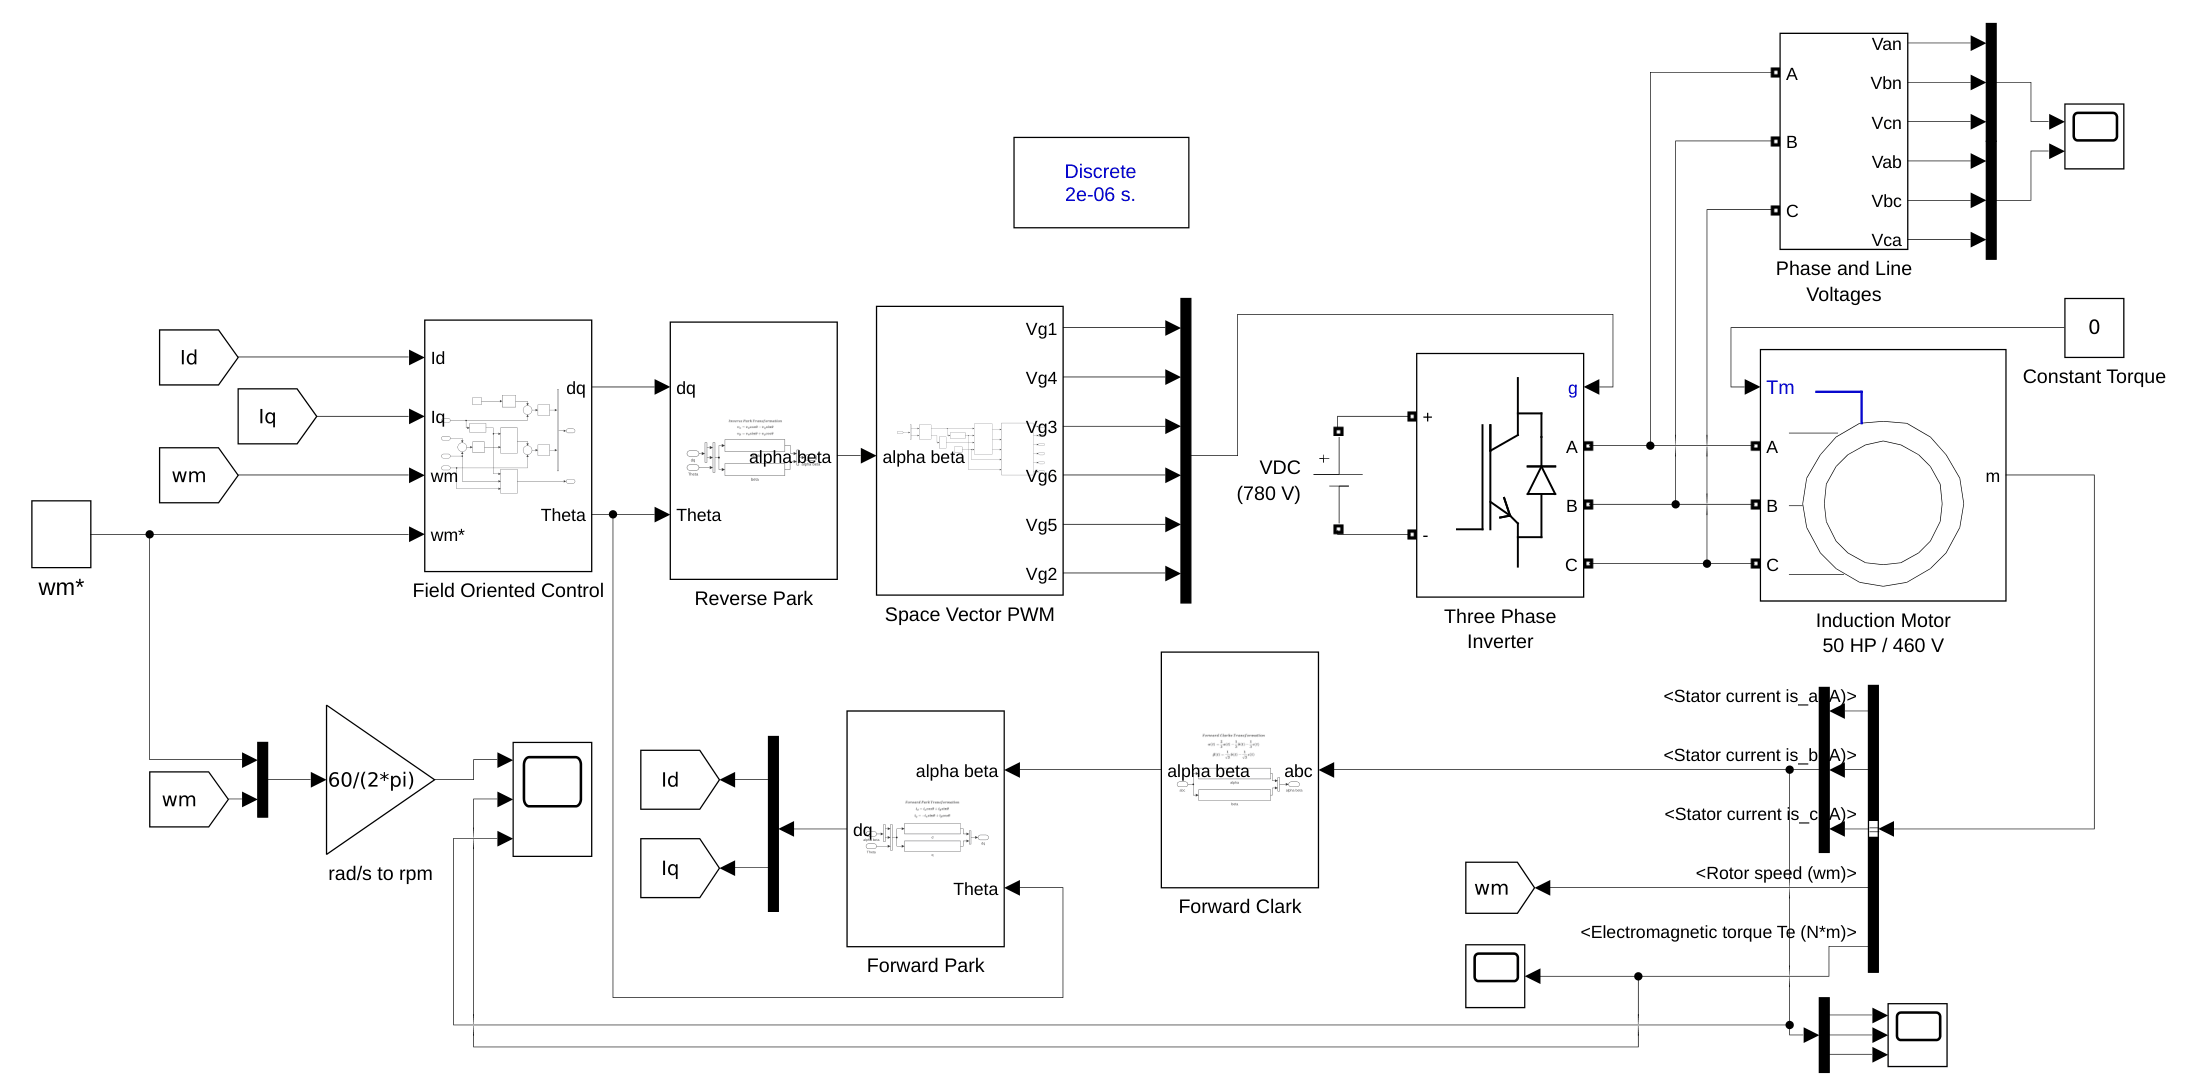
\includegraphics[width=0.8\textwidth]{VECTOR_CONTROL_FOC_OF_IM-01.png}
    \end{figure}
    \begin{itemize}
        \item \textbf{Outer Loop:} Speed regulation PI controller generating the torque command ($T_e^*$).
        \item \textbf{Inner Loop:} High-bandwidth PI current regulators ($i_d, i_q$).
        \item \textbf{Actuation:} Space Vector PWM (SVPWM) driving a 780V DC-link Three-Phase Inverter.
    \end{itemize}
\end{frame}

% --- Slide 4: Induction Motor Plant Parameters ---
\begin{frame}{The Induction Motor Plant Parameters}
    \textbf{Equivalent Circuit Specifications}
    \begin{columns}
        \begin{column}{0.5\textwidth}
            \begin{itemize}
                \item \textbf{Motor Ratings:} 50 HP (37.3 kW), 460 V, 50 Hz, 4-Pole (1500 RPM).
                \item \textbf{Electrical Parameters:}
                \begin{itemize}
                    \item Stator Res. ($R_s$): $0.087\ \Omega$
                    \item Rotor Res. ($R_r$): $0.228\ \Omega$
                    \item Mag. Ind. ($L_m$): $34.7\text{ mH}$
                \end{itemize}
            \end{itemize}
        \end{column}
        \begin{column}{0.5\textwidth}
            \textbf{Derived Self-Inductances:}
            \begin{align*}
                L_s &= L_{ls} + L_m = 34.8\text{ mH} \\
                L_r &= L_{lr} + L_m = 35.5\text{ mH}
            \end{align*}
            \textbf{Rotor Time Constant:}
            \begin{equation*}
                \tau_r = \frac{L_r}{R_r} = 0.1557\text{ s}
            \end{equation*}
        \end{column}
    \end{columns}
\end{frame}

% --- Slide 5: Dynamic Modeling & Mechanical System ---
\begin{frame}{Dynamic Modeling \& Mechanical System}
    \textbf{Understanding the Mechanical Transfer Function}
    \vspace{0.3cm}
    \begin{itemize}
        \item \textbf{Mechanical Equation of Motion:} 
        $$T_e - T_L = J\frac{d\omega_m}{dt} + F\omega_m$$
        \item \textbf{Mechanical Parameters:} Inertia ($J$) = $0.662\text{ kg}\cdot\text{m}^2$, Friction ($F$) = $0.1\text{ Nms/rad}$.
        \item \textbf{Laplace Domain Transfer Function:}
        $$\frac{\omega_m(s)}{T_e(s)} = \frac{1}{0.662s + 0.1}$$
        \item \textbf{Significance:} The high inertia acts as a natural low-pass filter, naturally attenuating high-frequency torque ripples generated by the SVPWM inverter.
    \end{itemize}
\end{frame}

% --- Slide 6: Coordinate Transformations Intro ---
\begin{frame}{Coordinate Transformations - The Core Concept}
    \textbf{Resolving the AC Control Dilemma}
    \vspace{0.3cm}
    \begin{itemize}
        \item \textbf{The Problem:} Standard PI controllers suffer from finite bandwidth limits and cannot track time-varying sinusoidal AC signals without steady-state amplitude and phase errors.
        \item \textbf{The Solution:} Mathematical spatial projections. 
        \item By transforming variables into a synchronously rotating reference frame ($d-q$), FOC mathematically forces these alternating signals to appear as trackable, flat DC quantities.
        \item This allows our standard PI controllers to achieve zero steady-state error.
    \end{itemize}
\end{frame}

% --- Slide 7: Forward Clarke Transform ---
\begin{frame}{Forward Clarke Transform}
    \textbf{Stationary $3\phi \rightarrow 2\phi$ Projection}
    \begin{columns}
        \begin{column}{0.5\textwidth}
            \begin{itemize}
                \item Simplifies the 3-phase system by projecting currents ($i_a, i_b, i_c$) onto a 2D stationary orthogonal frame ($\alpha-\beta$).
                \item Uses the amplitude-invariant matrix to preserve peak current amplitudes.
            \end{itemize}
            \begin{equation*}
                \begin{bmatrix} i_\alpha \\ i_\beta \end{bmatrix} = \frac{2}{3} \begin{bmatrix} 1 & -\frac{1}{2} & -\frac{1}{2} \\ 0 & \frac{\sqrt{3}}{2} & -\frac{\sqrt{3}}{2} \end{bmatrix} \begin{bmatrix} i_a \\ i_b \\ i_c \end{bmatrix}
            \end{equation*}
        \end{column}
        \begin{column}{0.5\textwidth}
            \begin{figure}
                \centering
                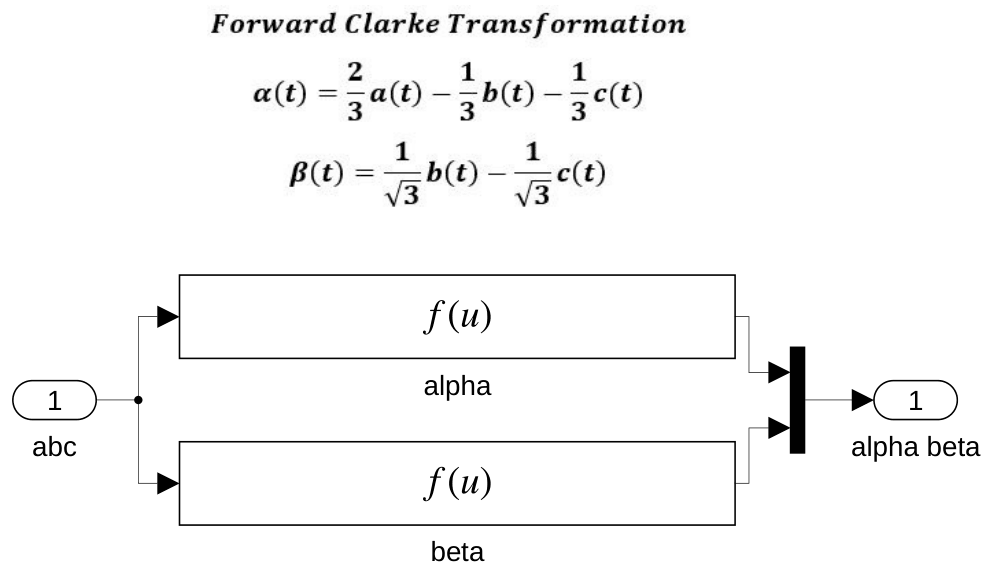
\includegraphics[width=\textwidth]{VECTOR_CONTROL_FOC_OF_IM-06.png}
            \end{figure}
        \end{column}
    \end{columns}
\end{frame}

% --- Slide 8: Forward Park Transform ---
\begin{frame}{Forward Park Transform}
    \textbf{Stationary $\alpha-\beta \rightarrow$ Rotating $d-q$ Projection}
    \begin{columns}
        \begin{column}{0.5\textwidth}
            \begin{itemize}
                \item Projects the stationary $\alpha-\beta$ frame onto a reference frame spinning at the electrical angular velocity of the rotor magnetic flux ($\theta_e$).
                \item Physically locks the observer's perspective to the spinning magnetic field, fully demodulating AC currents into DC.
            \end{itemize}
            \begin{equation*}
                \begin{bmatrix} i_d \\ i_q \end{bmatrix} = \begin{bmatrix} \cos\theta_e & \sin\theta_e \\ -\sin\theta_e & \cos\theta_e \end{bmatrix} \begin{bmatrix} i_\alpha \\ i_\beta \end{bmatrix}
            \end{equation*}
        \end{column}
        \begin{column}{0.5\textwidth}
            \begin{figure}
                \centering
                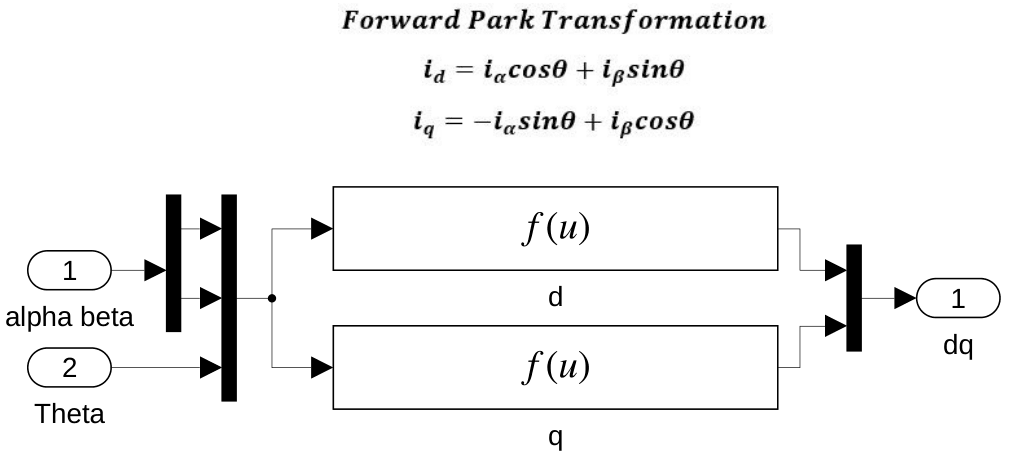
\includegraphics[width=\textwidth]{VECTOR_CONTROL_FOC_OF_IM-07.png}
            \end{figure}
        \end{column}
    \end{columns}
\end{frame}

% --- Slide 9: Reverse Park Transform ---
\begin{frame}{Reverse Park Transform}
    \textbf{Coordinate De-rotation for Actuation}
    \begin{columns}
        \begin{column}{0.5\textwidth}
            \begin{itemize}
                \item PI current regulators process DC error signals and output decoupling voltage commands ($v_d^*$ and $v_q^*$).
                \item Because the physical inverter operates in the stationary frame, these vectors must be de-rotated.
            \end{itemize}
            \begin{equation*}
                \begin{bmatrix} v_\alpha^* \\ v_\beta^* \end{bmatrix} = \begin{bmatrix} \cos\theta_e & -\sin\theta_e \\ \sin\theta_e & \cos\theta_e \end{bmatrix} \begin{bmatrix} v_d^* \\ v_q^* \end{bmatrix}
            \end{equation*}
        \end{column}
        \begin{column}{0.5\textwidth}
            \begin{figure}
                \centering
                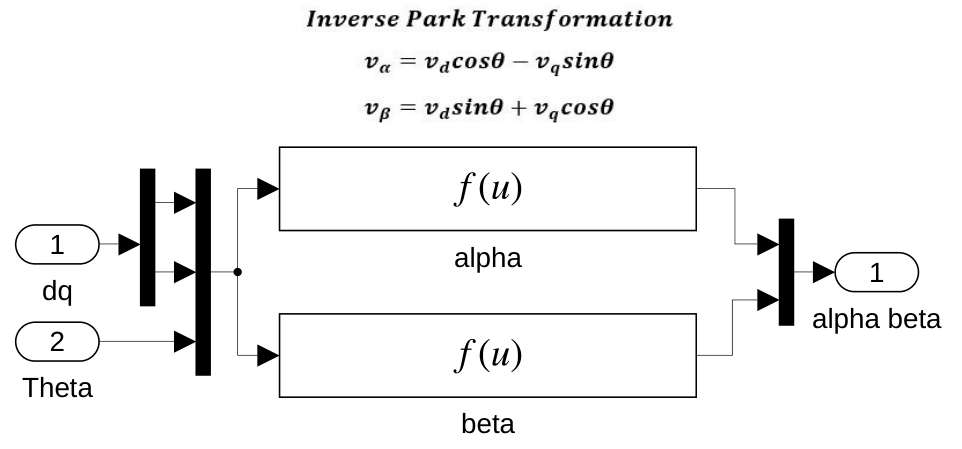
\includegraphics[width=\textwidth]{VECTOR_CONTROL_FOC_OF_IM-09.png}
            \end{figure}
        \end{column}
    \end{columns}
\end{frame}

% --- Slide 10: Flux Control ---
\begin{frame}{Flux Control (Direct-Axis Decoupling)}
    \textbf{Independent Magnetization Control}
    \begin{columns}
        \begin{column}{0.5\textwidth}
            \begin{itemize}
                \item The d-axis current ($i_{ds}$) strictly governs magnetization, analogous to field excitation in a DC motor.
                \item Under steady-state conditions ($\frac{d\psi_r}{dt} = 0$), the relationship simplifies to:
                $$i_{ds}^* = \frac{\psi_r^*}{L_m}$$
                \item For a nominal flux of $0.96\text{ Wb}$ and $L_m = 0.0347\text{ H}$, the reference current is firmly regulated to \textbf{$27.67\text{ A}$}.
            \end{itemize}
        \end{column}
        \begin{column}{0.5\textwidth}
            \begin{figure}
                \centering
                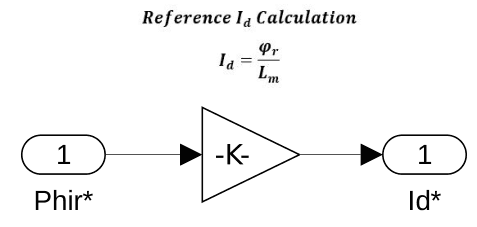
\includegraphics[width=\textwidth]{VECTOR_CONTROL_FOC_OF_IM-03.png}
            \end{figure}
        \end{column}
    \end{columns}
\end{frame}

% --- Slide 11: Torque Control ---
\begin{frame}{Torque Control (Quadrature-Axis Decoupling)}
    \textbf{Independent Active Force Control}
    \begin{columns}
        \begin{column}{0.5\textwidth}
            \begin{itemize}
                \item The q-axis current ($i_{qs}$) is maintained precisely at a 90$^\circ$ angle to the flux axis ($\psi_{qr} = 0$).
                \item \textbf{Decoupled Torque Equation:}
                $$T_e = \frac{3}{2}\left(\frac{P}{2}\right)\frac{L_m}{L_r}\psi_r i_{qs}$$
                \item Isolating $i_{qs}^*$ yields a direct torque constant:
                $$T_e = 2.8152\cdot i_{qs} \text{ N}\cdot\text{m}$$
            \end{itemize}
        \end{column}
        \begin{column}{0.5\textwidth}
            \begin{figure}
                \centering
                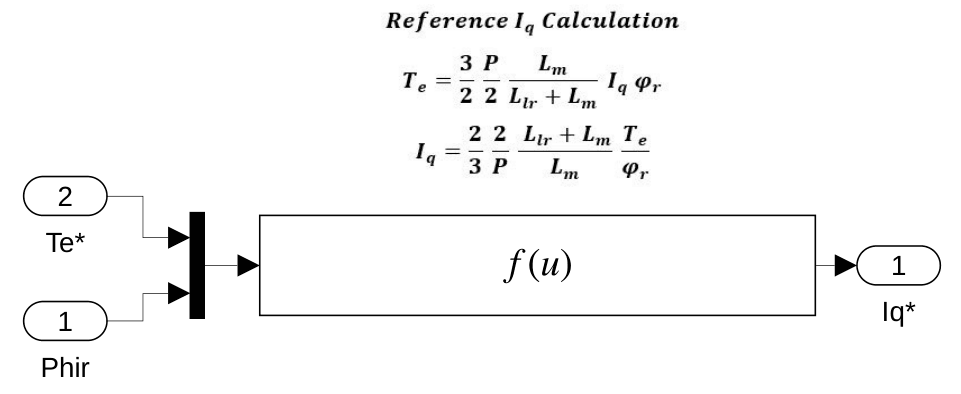
\includegraphics[width=\textwidth]{VECTOR_CONTROL_FOC_OF_IM-04.png}
            \end{figure}
        \end{column}
    \end{columns}
\end{frame}

% --- Slide 12: Computational Safeguards ---
\begin{frame}{Computational Safeguards in Digital FOC}
    \textbf{Preventing Division-by-Zero Singularities}
    \vspace{0.3cm}
    \begin{itemize}
        \item A critical engineering consideration occurs during motor startup ($t=0$) when the machine is completely unmagnetized ($\psi_r \approx 0$).
        \item Native execution of the $i_{qs}^*$ equation would cause a division-by-zero singularity, crashing the DSP or driving PI regulators into windup.
        \item \textbf{Solution:} The Simulink algorithm introduces a numerical perturbation ($\epsilon = 10^{-3}$) to the flux denominator:
        $$i_{qs}^* \propto \frac{T_e^*}{\psi_r + 10^{-3}}$$
        \item Keeps the starting current extremely high, but safely bounded.
    \end{itemize}
\end{frame}

% --- Slide 13: Slip and Flux Angle Synthesis ---
\begin{frame}{Slip and Flux Angle ($\theta_e$) Synthesis}
    \textbf{The Core of Indirect FOC (IFOC)}
    \begin{columns}
        \begin{column}{0.5\textwidth}
            \begin{itemize}
                \item IFOC mathematically synthesizes the flux angle using a feedforward slip calculation, avoiding fragile air-gap sensors.
                \item \textbf{Required Slip Frequency:}
                $$\omega_{sl} = \frac{L_m}{\tau_r} \cdot \frac{i_{qs}^*}{\psi_r^*}$$
                \item \textbf{Synchronous Speed:} 
                $$\omega_e = \omega_r + \omega_{sl}$$
            \end{itemize}
        \end{column}
        \begin{column}{0.5\textwidth}
            \begin{figure}
                \centering
                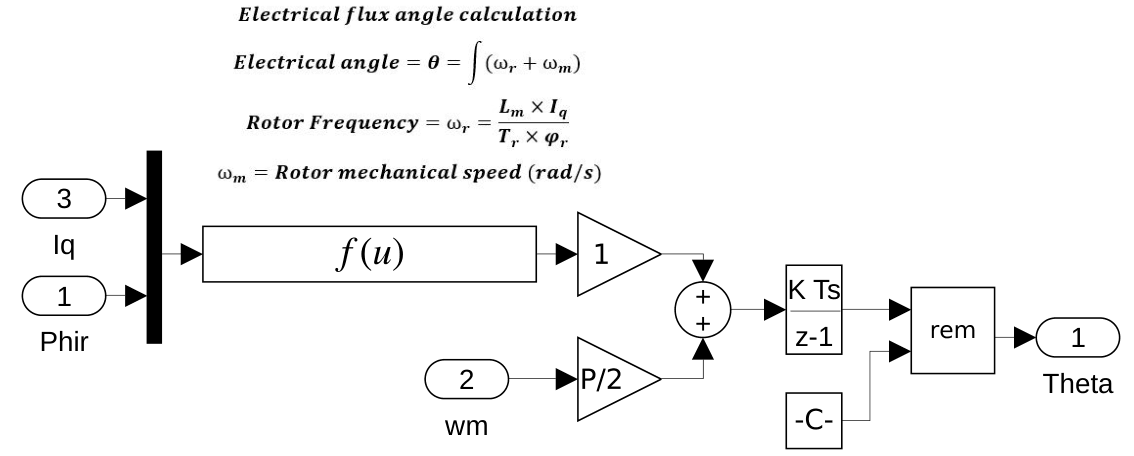
\includegraphics[width=\textwidth]{VECTOR_CONTROL_FOC_OF_IM-05.png}
            \end{figure}
        \end{column}
    \end{columns}
\end{frame}

% --- Slide 14: Discrete Integration for Angle ---
\begin{frame}{Discrete Integration for Angle ($\theta_e$)}
    \textbf{Digital Implementation Constraints}
    \vspace{0.3cm}
    \begin{itemize}
        \item The instantaneous rotor flux angle ($\theta_e$) must be calculated by integrating the synchronous speed continuously.
        \item Executed at the model's fundamental $2\mu\text{s}$ discrete sample time using Forward Euler:
        $$\theta_e[k] = (\theta_e[k-1] + \omega_e[k] \cdot T_s) \pmod{2\pi}$$
        \item The modulo $2\pi$ operator wraps the angle within $[0, 2\pi]$, preventing numerical overflow in DSP registers during continuous operation.
    \end{itemize}
\end{frame}

% --- Slide 15: Introduction to Space Vector PWM ---
\begin{frame}{Space Vector PWM (SVPWM)}
    \textbf{Connecting Mathematics to Power Electronics}
    \begin{figure}
        \centering
        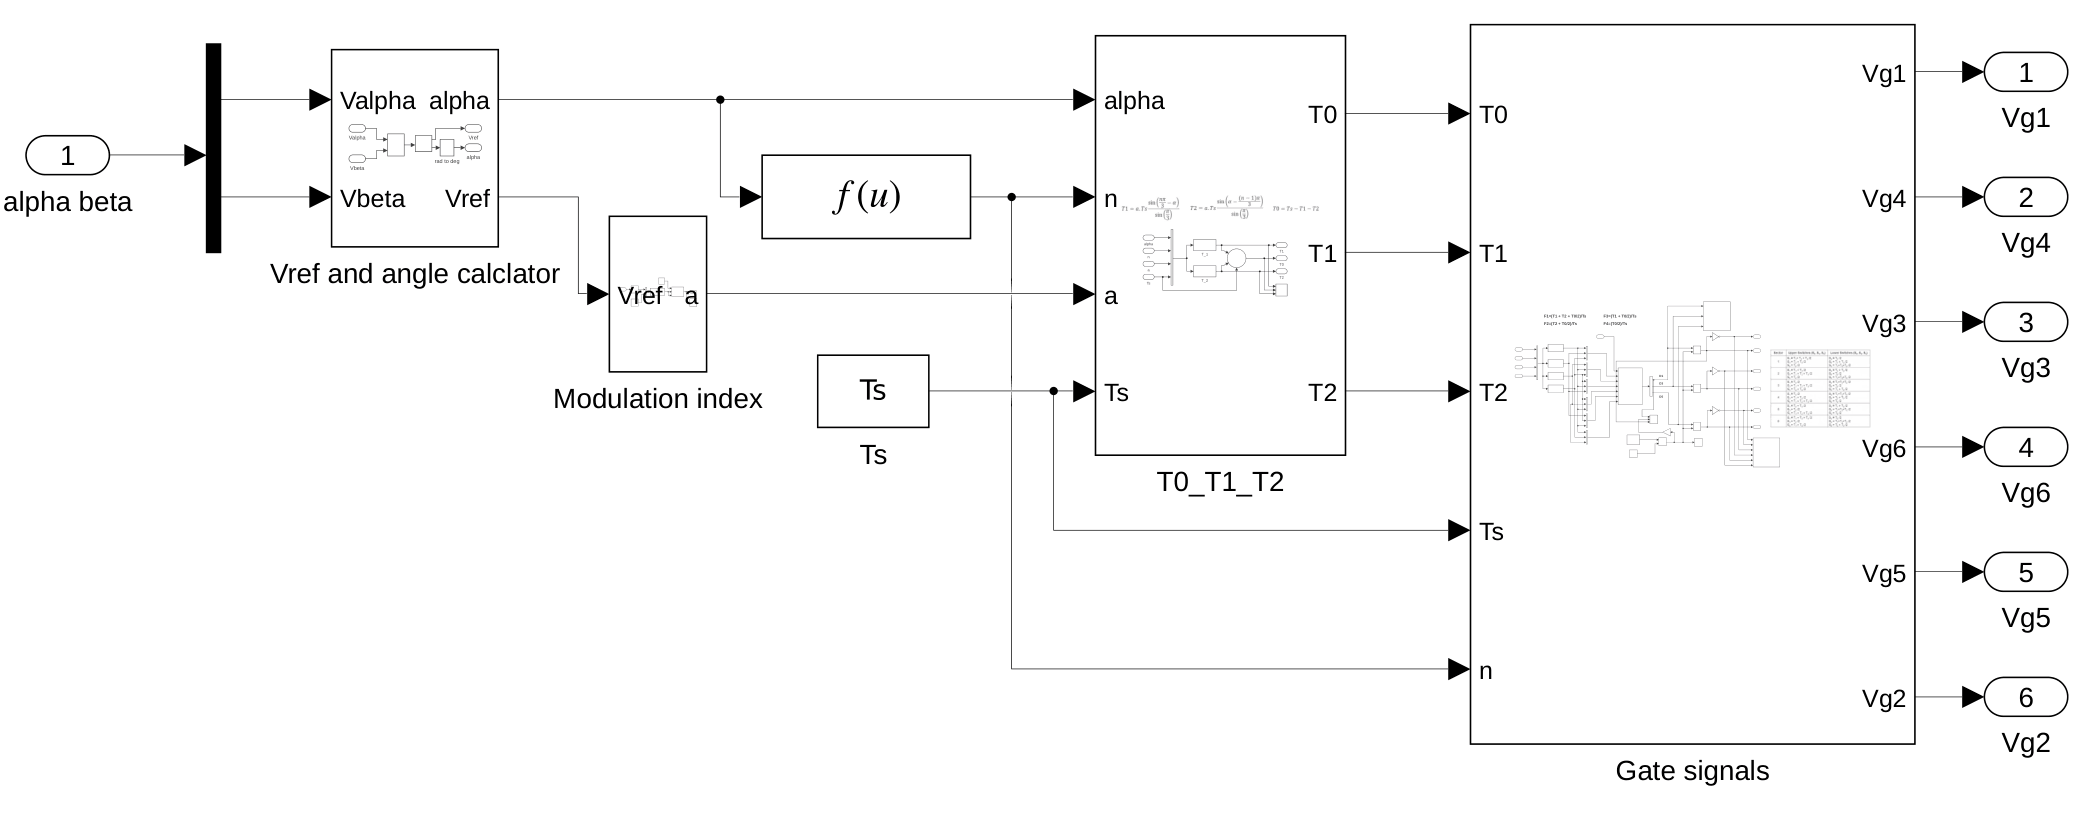
\includegraphics[width=0.85\textwidth]{VECTOR_CONTROL_FOC_OF_IM-10.png}
    \end{figure}
    \begin{itemize}
        \item Translates continuous $v_\alpha^*$ and $v_\beta^*$ commands into discrete transistor switching signals for the 780 V DC-link inverter.
        \item \textbf{Why SVPWM?} Injects zero-sequence voltages, enhancing DC Bus Utilization by $\approx 15.47\%$ and drastically minimizing Total Harmonic Distortion (THD).
    \end{itemize}
\end{frame}

% --- Slide 16: SVPWM Reference Synthesis ---
\begin{frame}{SVPWM Algorithm - Reference Synthesis}
    \textbf{Calculating Magnitude and Modulation Index}
    \begin{columns}
        \begin{column}{0.5\textwidth}
            \begin{itemize}
                \item Converts stationary commands into a rotating polar vector:
                $$|\vec{V}_{ref}| = \sqrt{(v_\alpha^*)^2 + (v_\beta^*)^2}$$
                $$\theta_{ref} = \arctan\left(\frac{v_\beta^*}{v_\alpha^*}\right)$$
                \item \textbf{Modulation Index ($a$):} Bounded by a saturation switch ($\le 0.866$) to prevent deep overmodulation and distortion.
            \end{itemize}
        \end{column}
        \begin{column}{0.5\textwidth}
            \begin{figure}
                \centering
                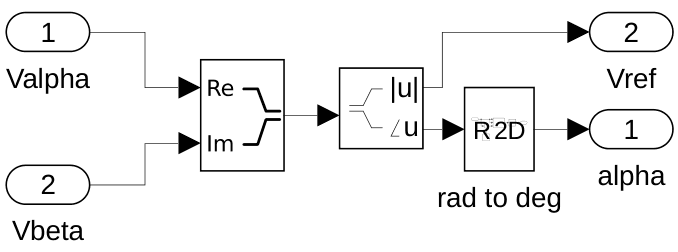
\includegraphics[width=\textwidth]{VECTOR_CONTROL_FOC_OF_IM-14.png}
            \end{figure}
            \begin{figure}
                \centering
                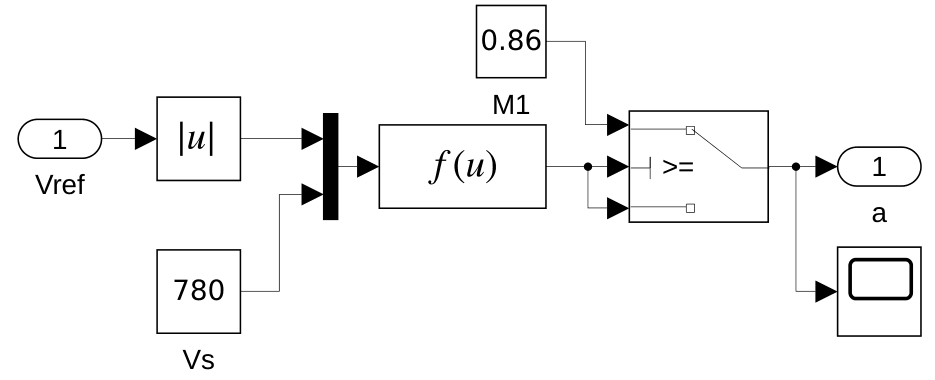
\includegraphics[width=\textwidth]{VECTOR_CONTROL_FOC_OF_IM-12.png}
            \end{figure}
        \end{column}
    \end{columns}
\end{frame}

% --- Slide 17: SVPWM Dwell Times ---
\begin{frame}{SVPWM Algorithm - Dwell Times}
    \textbf{Applying the Volt-Second Balance Principle}
    \begin{columns}
        \begin{column}{0.5\textwidth}
            \begin{itemize}
                \item Synthesizes the target vector by time-averaging active vectors ($T_1, T_2$) and the zero vector ($T_0$).
                \item \textbf{Equations:}
                \begin{align*}
                    T_1 &= a \cdot T_s \frac{\sin(\frac{n\pi}{3} - \alpha)}{\sin(\frac{\pi}{3})} \\
                    T_2 &= a \cdot T_s \frac{\sin(\alpha - \frac{(n-1)\pi}{3})}{\sin(\frac{\pi}{3})} \\
                    T_0 &= T_s - T_1 - T_2
                \end{align*}
            \end{itemize}
        \end{column}
        \begin{column}{0.5\textwidth}
            \begin{figure}
                \centering
                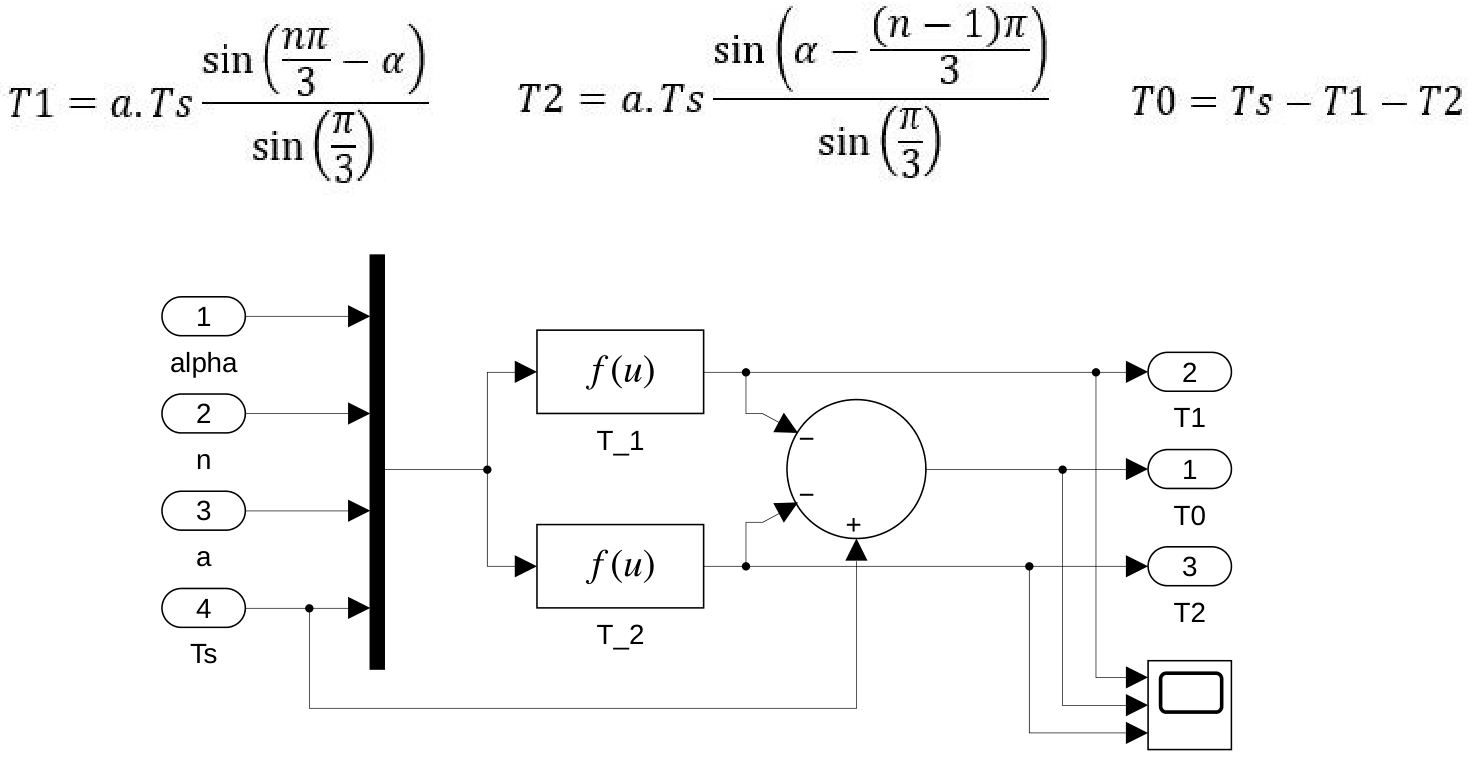
\includegraphics[width=\textwidth]{VECTOR_CONTROL_FOC_OF_IM-13.png}
            \end{figure}
        \end{column}
    \end{columns}
\end{frame}

% --- Slide 18: Transient Tracking Results ---
\begin{frame}{Simulation Results: Transient Tracking}
    \textbf{Validating Dynamic Response}
    \begin{columns}
        \begin{column}{0.4\textwidth}
            \begin{itemize}
                \item Motor tracks aggressive staircase speed references flawlessly.
                \item Decoupling verified: Torque ($T_e$) acts directly and instantaneously to speed errors.
                \item Peaks near $\approx 830\text{ N}\cdot\text{m}$ during acceleration; drops to $\approx -680\text{ N}\cdot\text{m}$ for regenerative braking.
            \end{itemize}
        \end{column}
        \begin{column}{0.6\textwidth}
            \begin{figure}
                \centering
                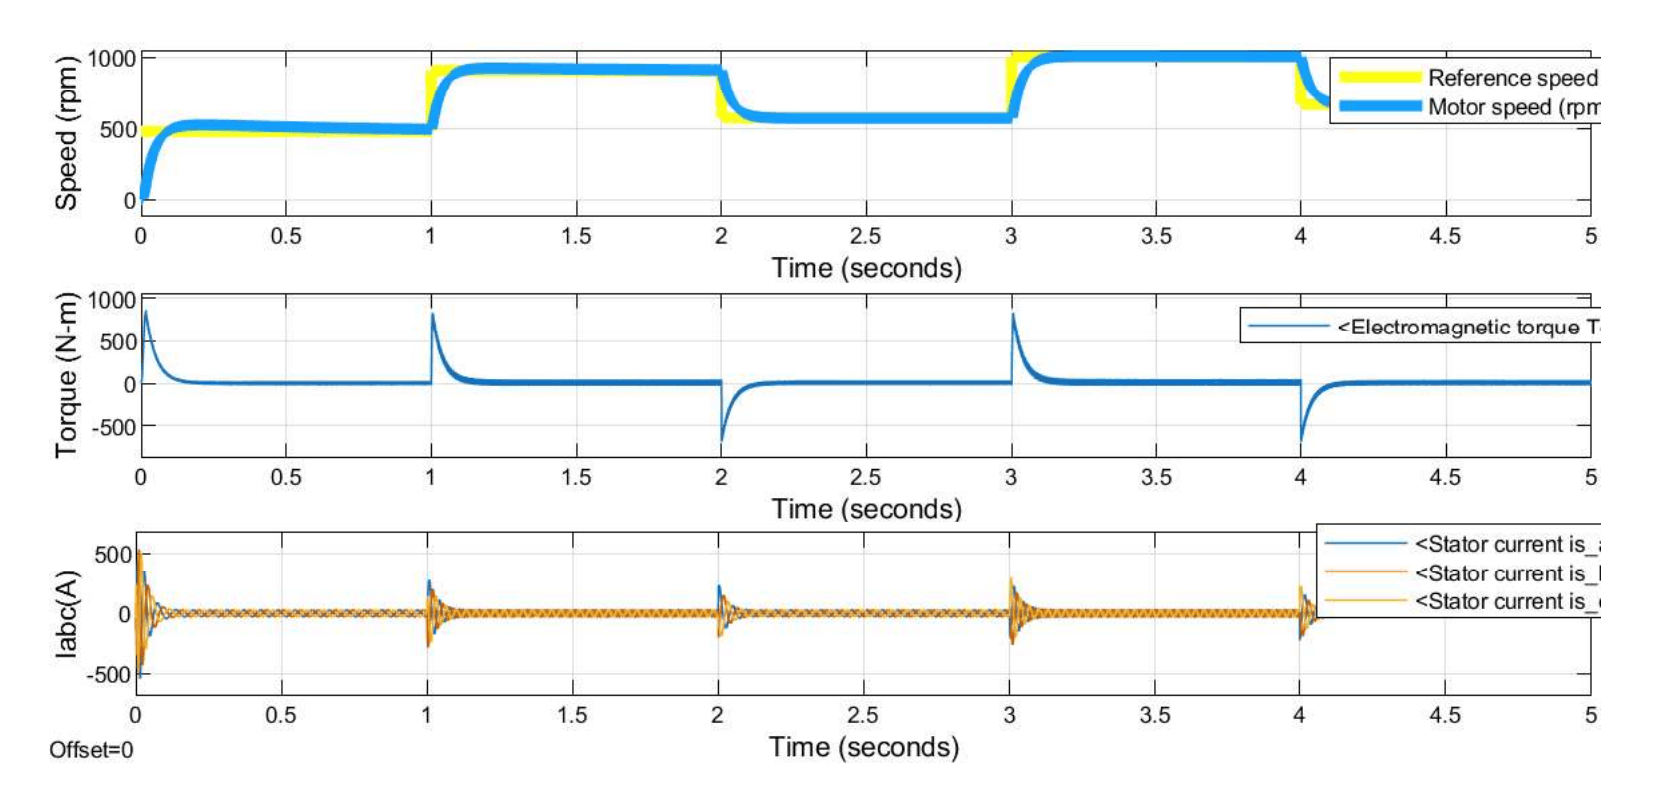
\includegraphics[width=\textwidth]{7.png}
            \end{figure}
        \end{column}
    \end{columns}
\end{frame}

% --- Slide 19: Current Regulation Results ---
\begin{frame}{Simulation Results: Current Regulation}
    \textbf{Validating the Inner Control Loops}
    \begin{columns}
        \begin{column}{0.4\textwidth}
            \begin{itemize}
                \item Steady-state phase currents drop to a tiny magnetizing envelope.
                \item During speed transients, current envelope flares symmetrically to peak amplitudes near $500\text{ A}$.
                \item Accurate translation of PI torque commands without unstable overcurrent limits.
            \end{itemize}
        \end{column}
        \begin{column}{0.6\textwidth}
            \begin{figure}
                \centering
                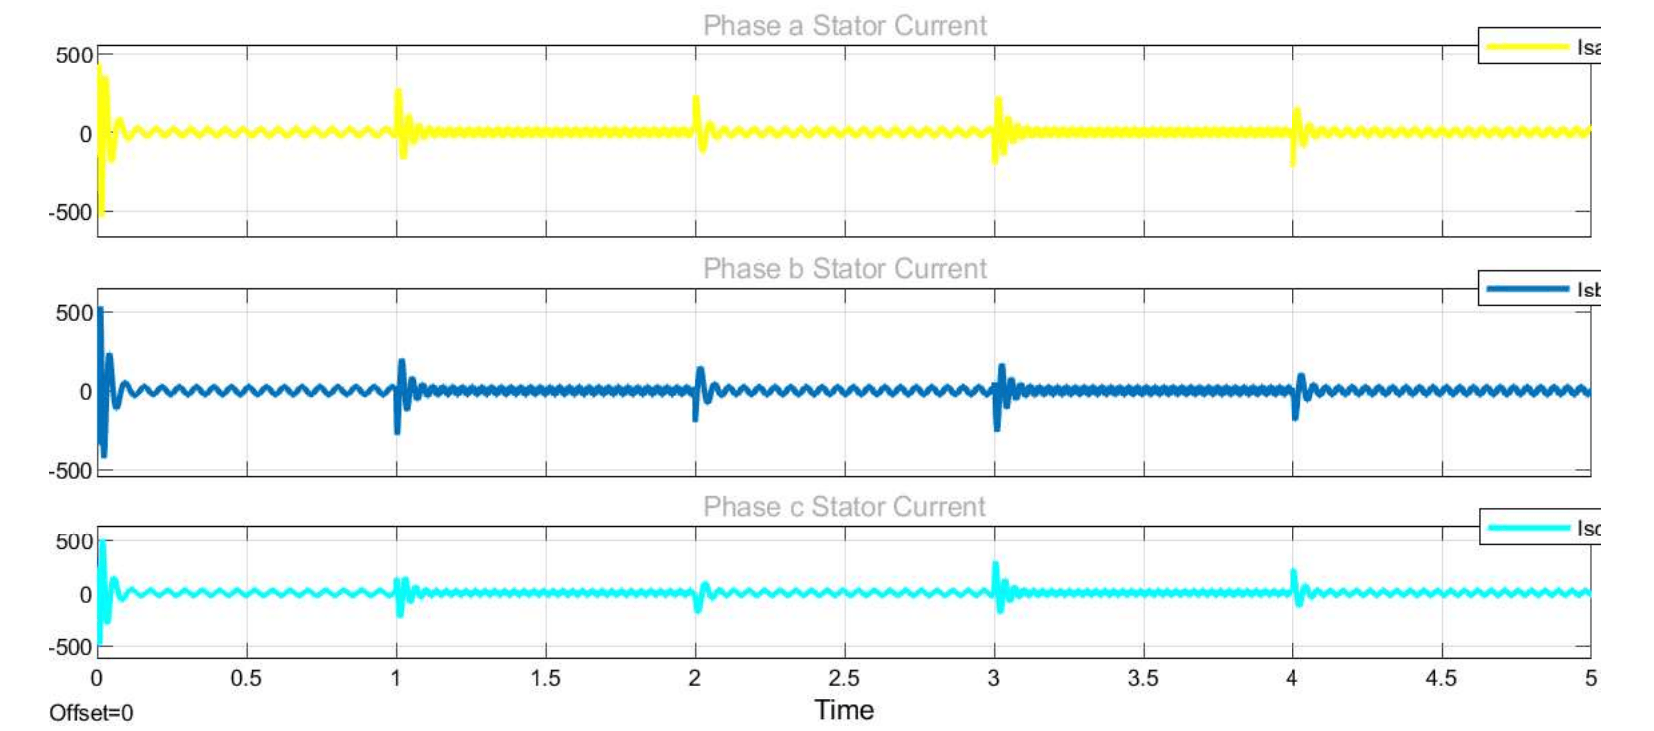
\includegraphics[width=\textwidth]{23.png}
            \end{figure}
        \end{column}
    \end{columns}
\end{frame}

% --- Slide 20: Conclusion & Future Scope ---
\begin{frame}{Conclusion \& Future Scope}
    \textbf{Conclusion:}
    \begin{itemize}
        \item Validated a functionally complete "digital twin" of an industrial IFOC drive.
        \item Demonstrated how non-linear, multi-variable AC machines can be transformed into decoupled, linear systems yielding DC-like performance.
    \end{itemize}
    \vspace{0.3cm}
    \textbf{Future Scope:}
    \begin{itemize}
        \item \textbf{Sensorless Control:} Implement Model Reference Adaptive Systems (MRAS) to eliminate the physical speed encoder.
        \item \textbf{Online Parameter Identification:} Dynamically estimate rotor resistance ($R_r$) to prevent vector detuning caused by thermal heating.
        \item \textbf{Field Weakening:} Actively attenuate $i_{ds}$ to push the machine into the constant-power region above base speed.
    \end{itemize}
\end{frame}

\end{document}